\documentclass{article}
\usepackage[utf8]{inputenc}
\usepackage[T1]{fontenc}
\usepackage[utf8]{inputenc}
\usepackage[norsk]{babel}
\usepackage{amsmath}
\usepackage{hyperref}
\usepackage{enumerate}
\usepackage{graphicx}
\usepackage{listings}
\usepackage{color}
\usepackage{gensymb}
\usepackage{subfig}
\definecolor{codegreen}{rgb}{0,0.6,0}
\definecolor{codegray}{rgb}{0.5,0.5,0.5}
\definecolor{codepurple}{rgb}{0.58,0,0.82}
\definecolor{backcolour}{rgb}{0.95,0.95,0.92}
\setlength{\parindent}{0pt}
\lstdefinestyle{mystyle}{
    backgroundcolor=\color{backcolour},
    commentstyle=\color{codegreen},
    keywordstyle=\color{magenta},
    numberstyle=\tiny\color{codegray},
    stringstyle=\color{codepurple},
    basicstyle=\footnotesize,
    breakatwhitespace=false,
    breaklines=true,
    captionpos=b,
    keepspaces=true,
    numbers=left,
    numbersep=5pt,
    showspaces=false,
    showstringspaces=false,
    showtabs=false,
tabsize=2}
\lstset{style=mystyle}

\title{Oblig1 INF2270}
\author{mathiaki}
\date{February 2017}

\begin{document}

\maketitle

\newpage
\tableofcontents
\newpage

\section{Texture discription}
First, when i describe the different textures, i will index the different images in the following way: (the same is true for the program)\\
\begin{verbatim}
 img0        img1      img0     img1
|---|---| |---|---| |-------| |-------|
| 0 | 1 | | 4 | 5 | |       | |       |
|---|---| |---|---| |   8   | |   9   |
| 2 | 3 | | 6 | 7 | |       | |       |
|---|---| |---|---| |-------| |-------|

\end{verbatim}

This means i will start in the top left corner of mosaic1 and and in the bottom right corner of mosaic2. In the program 8 and 9 is reserved for the whole mosaic1 and mosaic2 respectivly. 

\newpage

\subsection{Texture 0}
\textbf{Caracteristics:}\\
Textue is mainly random noise. Somewhere in the texture you get some patters that looks like holes. \\

\textbf{Texture Direction}\\
There are a sligt movement in the \textbf{3pi/4 rad} direction, although as mentioned, som sicular patterns can be observed. \\

\textbf{Frequency} \\
The crevasas is on a rough average 10px in diameter, and the edges beween them is closer to 4px.\\ 


\textbf{Varience}\\
If we look at the histogram, we can see that it is one of the textures with the least varience. We do have some peaks that drives down the varience a bit\\

\textbf{Homogenity}\\
The texture is has very few homogen areas.\\

\textbf{Texture element size}\\
As mentioned, alement size is hard to determine.

\begin{figure}[h]%
	\centering
    \subfloat[IMG 0]{{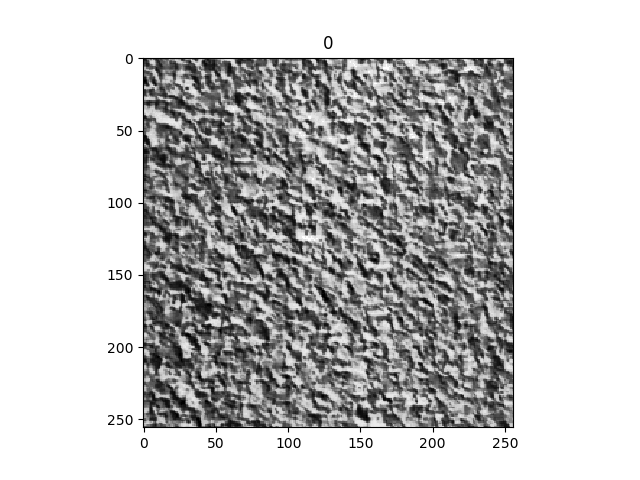
\includegraphics[width=5.5cm]{0.png} }}%
    \qquad
    \subfloat[Hist IMG 0]{{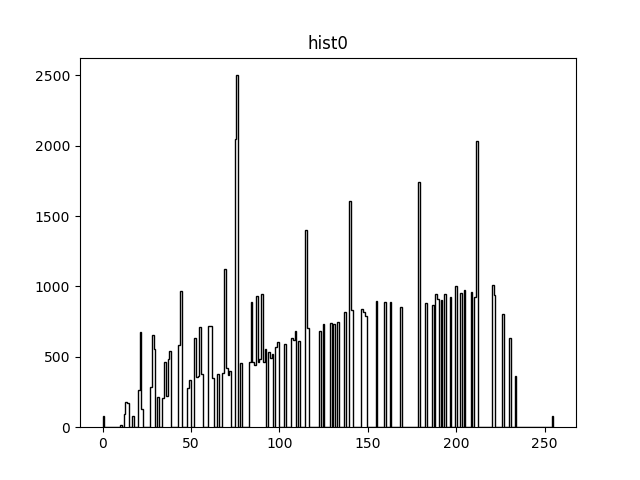
\includegraphics[width=5.5cm]{hist0.png} }}%
    \caption{Texture with histogram}%
    \label{fig:IMG0}%
\end{figure}



\newpage
\subsection{Texture 1}
\textbf{Caracteristics:}\\
Textue has a clearer pattern of squares that is roughly 8 px wide and high.
It is also some radom noise on top of the texture. 
\\

\textbf{Texture Direction}\\
The texture direction is almost horizontal (and verical), with a slight scewe.\\

\textbf{Frequency} \\
The frequency of the texture is equal to the length of the squares.
\\ 


\textbf{Varience}\\
The istogram is fairly balanced, so the varience is in the middle if the spectrum. Especially compared to \ref{fig:IMG2} \\

\textbf{Homogenity}\\
The texture is has very few homogene areas.\\

\textbf{Texture element size}\\
As mentioned, the quares has a diameter of approximently 7 px.


\begin{figure}[h]%
	\centering
    \subfloat[IMG 1]{{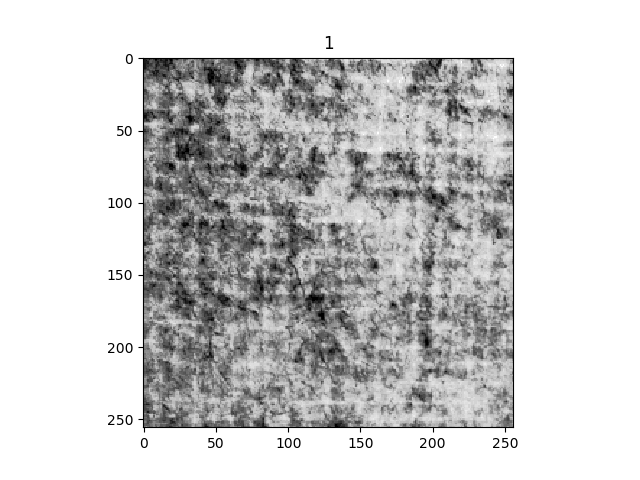
\includegraphics[width=5.5cm]{1.png} }}%
    \qquad
    \subfloat[Hist IMG 1]{{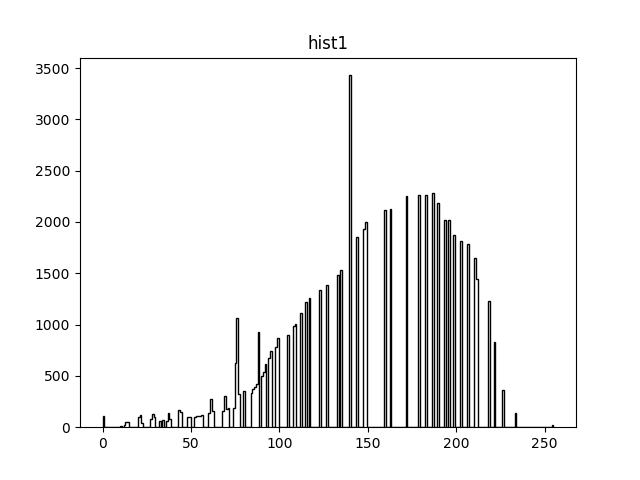
\includegraphics[width=5.5cm]{hist1.png} }}%
    \caption{Texture with histogram}%
    \label{fig:IMG1}%
\end{figure}

\newpage
\subsection{Texture 2}
\textbf{Caracteristics:}\\
The texture is a series of lines that face in roughly the same direction.
\\

\textbf{Texture Direction}\\
The mayority of the stripes has an angle of 100\textbf{deg}.
\\ 
 
\textbf{Frequency} \\
The frequency of the pattern, diagonally to the lines is \textbf{X} pixels.
\\ 


\textbf{Varience}\\
This pattern has a small varience, probably the smallest.
\\

\textbf{Homogenity}\\
The texture is has very few homogene areas.\\

\textbf{Texture element size}\\
The element size is only a few pixels wide, and \textbf{X} pixels high.


\begin{figure}[h]%
	\centering
    \subfloat[IMG 2]{{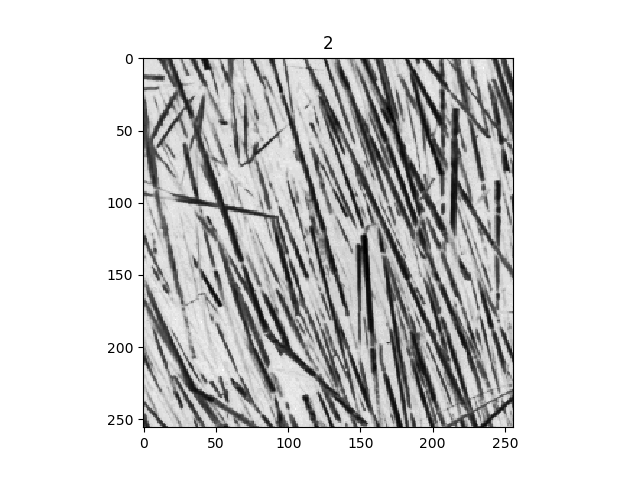
\includegraphics[width=5.5cm]{2.png} }}%
    \qquad
    \subfloat[Hist IMG 2]{{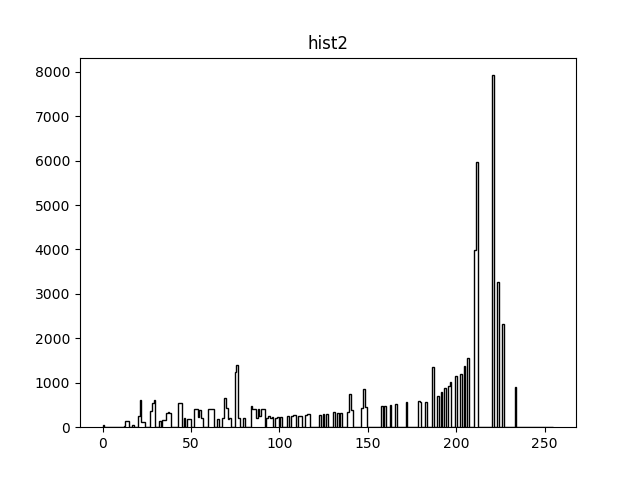
\includegraphics[width=5.5cm]{hist2.png} }}%
    \caption{Texture with histogram}%
    \label{fig:IMG2}%
\end{figure}

\newpage

\subsection{Texture 3}
\textbf{Caracteristics:}\\
This seems like another white noice texture.\\

\textbf{Texture Direction}\\
There are no clear direction in the texture. This and the first one is isotropic textures.
\\ 
 
\textbf{Frequency} \\
It is hard to say anyting about the frequency, but a rough guess might be 2-3px\\ 


\textbf{Varience}\\
This pattern has a low variance, but the pixel value ~75 upping the variance.
\\

\textbf{Homogenity}\\
The texture is not homogene, nor does it have any homogene areas.\\

\textbf{Texture element size}\\
\textbf{WIP}
\\

\begin{figure}[h]%
	\centering
    \subfloat[IMG 3]{{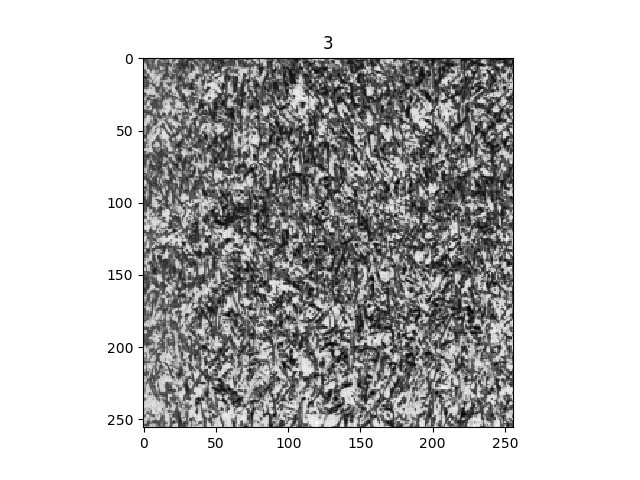
\includegraphics[width=5.5cm]{3.png} }}%
    \qquad
    \subfloat[Hist IMG 3]{{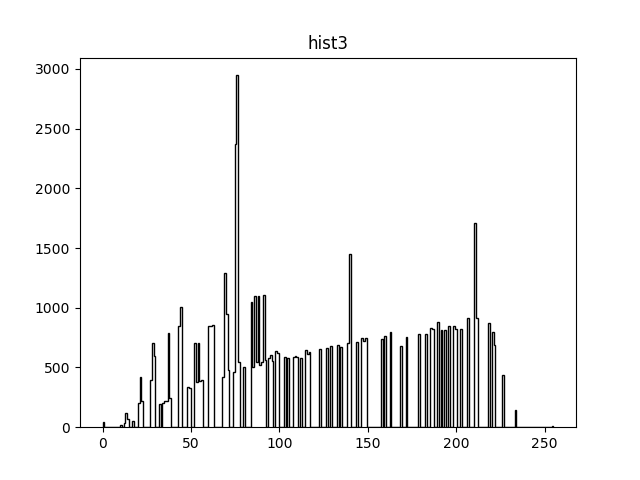
\includegraphics[width=5.5cm]{hist3.png} }}%
    \caption{Texture with histogram}%
    \label{fig:IMG3}%
\end{figure}
\newpage

\subsection{Texture 4}
\textbf{Caracteristics:}\\
This texture has a clear pattern 

\textbf{Texture Direction}\\
There are no clear direction in the texture. This and the first one is isotropic textures.
\\ 
 
\textbf{Frequency} \\
It is hard to say anyting about the frequency, but a rough guess might be 2-3px\\ 


\textbf{Varience}\\
This pattern has a low variance, but the pixel value ~75 upping the variance.
\\

\textbf{Homogenity}\\
The texture is not homogene, nor does it have any homogene areas.\\

\textbf{Texture element size}\\
\textbf{WIP}
\\

\begin{figure}[h]%
	\centering
    \subfloat[IMG 4]{{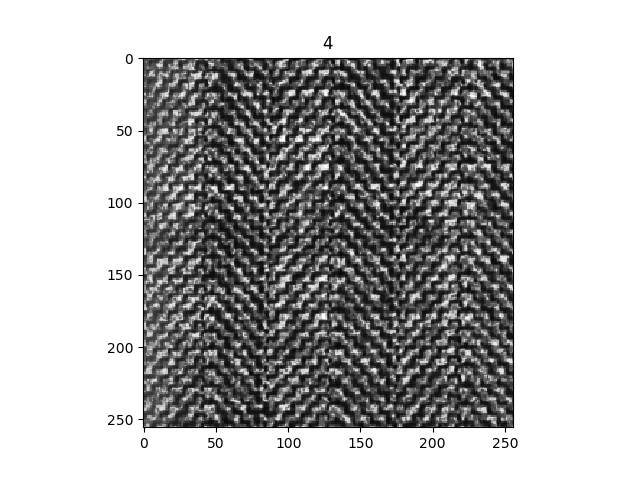
\includegraphics[width=5.5cm]{4.png} }}%
    \qquad
    \subfloat[Hist IMG 4]{{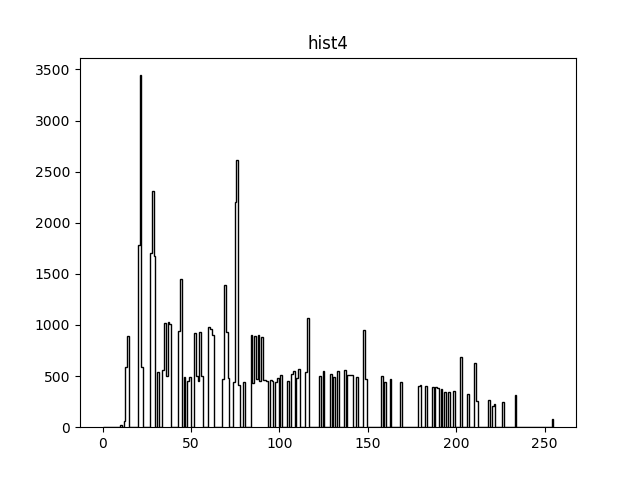
\includegraphics[width=5.5cm]{hist4.png} }}%
    \caption{Texture with histogram}%
    \label{fig:IMG4}%
\end{figure}
\newpage


\subsection{Texture 5}
\textbf{disc of texture}
\textbf{disc of texture}
\textbf{disc of texture}
\textbf{disc of texture}
\textbf{disc of texture}
\textbf{disc of texture}
\begin{figure}[h!]
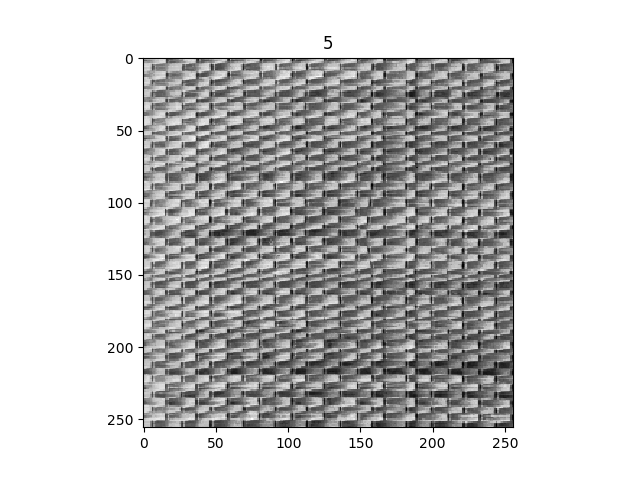
\includegraphics[scale=0.5]{5.png}
\end{figure}

\subsection{Texture 6}
\textbf{disc of texture}
\textbf{disc of texture}
\textbf{disc of texture}
\textbf{disc of texture}
\textbf{disc of texture}
\textbf{disc of texture}
\begin{figure}[h!]
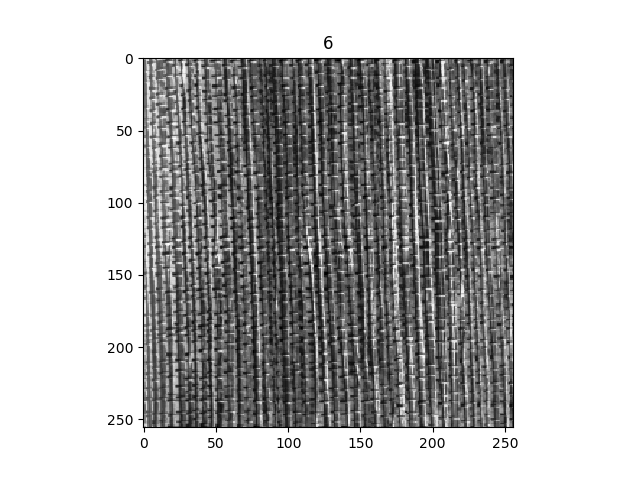
\includegraphics[scale=0.5]{6.png}
\end{figure}

\newpage

\subsection{Texture 7}
\textbf{disc of texture}
\textbf{disc of texture}
\textbf{disc of texture}
\textbf{disc of texture}
\textbf{disc of texture}
\textbf{disc of texture}
\begin{figure}[h!]
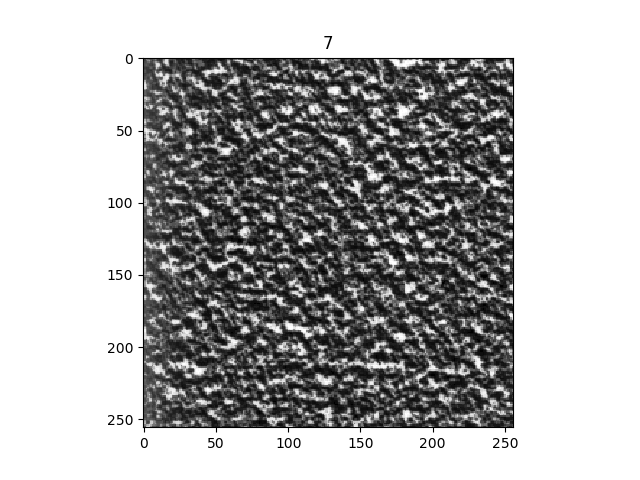
\includegraphics[scale=0.5]{7.png}
\end{figure}

\section{2}



\end{document}\\

